% =============================================================
% EK A: Sayı Sistemleri ve Kodlama
% =============================================================
\chapter{Sayı Sistemleri ve Kodlama}
\label{ch:sayi-sistemleri}
%\bolumfoto{gorseller/ekA-foto.jpg}{Fotoğraf Açıklaması}

Bu ekte, bilgisayar mimarisinin temelini oluşturan sayı sistemleri ve kodlama yöntemleri ele alınmaktadır. İkilik taban, taban dönüşümleri, işaretli sayı gösterimleri ve karakter kodlama gibi konular, kitabın ana bölümlerinde sıkça başvurulan ön bilgileri oluşturur.

% =====================================================
\section{İkilik Tabanda İşlemler}
\label{sec:ikilik-taban}

Günlük hayatta 10'luk tabanı kullanırız çünkü on ayrı rakamımız (0--9) vardır. İkilik taban\index{ikilik taban} ise yalnızca iki rakamdan --- 0 ve 1 --- oluşur. Bu tabanda ``2'' rakamı yoktur; tıpkı 10'luk tabanda ``10'' diye tek bir rakam olmadığı gibi. Sayısal devrelerin doğal dili ikilik taban olduğu için bilgisayar mimarisinin temelini oluşturur.

\subsection{Taban Değiştirme İşlemleri}

Değişik sayı tabanlarında gösterilen sayıları 10'luk tabana çevirmek için, basamakların sayı içerisindeki değerlerini hesaplamayı sağlayan çözümleme yöntemi kullanılır. Bir sayı çözümlenirken, $i$. basamaktaki sayı için $b_i$ ve taban değeri için $t$ kullanıldığında, tabanın $(i-1)$. kuvveti $b_i$ sayısı ile çarpılır ve sayının 10'luk tabandaki değeri, ortaya çıkan ara çarpımlar toplanarak hesaplanır.

İkilik tabanda yazılmış sayıların onluk tabana çevrilmesinde, her basamaktaki sayı bulunduğu basamak değerini belirleyen ikinin kuvveti ile çarpılır ve bütün basamaklardan elde edilen sonuçlar toplanır.

\begin{ornek}[A.1]
İkilik tabandaki $1010011$ sayısını 10'luk tabana çevirin.

\textbf{Çözüm:}
\begin{align*}
(1010011)_2 &= 1\times 2^6 + 0\times 2^5 + 1\times 2^4 + 0\times 2^3 + 0\times 2^2 + 1\times 2^1 + 1\times 2^0 \\
&= 64 + 0 + 16 + 0 + 0 + 2 + 1 \\
&= (83)_{10}
\end{align*}
\end{ornek}

\begin{ornek}[A.2]
İkilik tabandaki $100101010$ sayısının 10'luk tabanda değeri nedir?

\textbf{Çözüm:}
\begin{align*}
(100101010)_2 &= 1\times 2^8 + 0\times 2^7 + 0\times 2^6 + 1\times 2^5 + 0\times 2^4 + 1\times 2^3 + 0\times 2^2 + 1\times 2^1 + 0\times 2^0 \\
&= 256 + 32 + 8 + 2 \\
&= (298)_{10}
\end{align*}
\end{ornek}

Sayılar onluk tabandan ikilik tabana çevrilmek istendiğinde, sayının içerisinde ikinin üssü olabilecek değerler aranır. Sayıdan küçük ve ikinin üzeri olan en büyük değer bulunduğunda, sonuçta ortaya çıkacak ikilik tabandaki sayının ilgili basamağına 1 değeri verilir ve sayıdan ikinin üssü olarak bulunan değer çıkarılır. Bu işlem tüm basamaklar için yinelenir.

\begin{ornek}[A.3]
$(83)_{10}$ sayısını çıkarma yöntemini kullanarak ikilik tabana çevirin.

\textbf{Çözüm:}

\begin{table}[H]
\centering
\begin{tabular}{ll}
\toprule
\textbf{İşlem Adımı} & \textbf{İkilik Tabandaki Sayı} \\
\midrule
$(83)_{10} - 2^6 = 19$ & 1 \\
$19 < 2^5$ & 10 \\
$19 - 2^4 = 3$ & 101 \\
$3 < 2^3$ & 1010 \\
$3 < 2^2$ & 10100 \\
$3 - 2^1 = 1$ & 101001 \\
$1 - 2^0 = 0$ & 1010011 \\
\bottomrule
\end{tabular}
\end{table}
\end{ornek}

Onluk tabandaki bir sayıyı ikilik tabana çevirmek için sayıyı sürekli ikiye bölerek kalana bakma yöntemi de kullanılabilir.

\begin{ornek}[A.4]
$(83)_{10}$ sayısını ikiye bölme yöntemini kullanarak ikilik tabana çevirin.

\textbf{Çözüm:}

\begin{table}[H]
\centering
\begin{tabular}{ll}
\toprule
\textbf{İşlem Adımı} & \textbf{Kalan} \\
\midrule
$83 / 2 = 41$ & 1 \\
$41 / 2 = 20$ & 1 \\
$20 / 2 = 10$ & 0 \\
$10 / 2 = 5$ & 0 \\
$5 / 2 = 2$ & 1 \\
$2 / 2 = 1$ & 0, Sonuç $= 1$ \\
\bottomrule
\end{tabular}
\end{table}

Bölme işlemlerinin ardından, son bölme işleminin sonucu en büyük basamağı ve bölme işlemlerinin kalanları diğer basamakları oluşturacak biçimde kalanlar sırayla yazılır ve sonuç $(83)_{10} = (1010011)_2$ olarak bulunur.
\end{ornek}

\subsection{İkilik Tabanda Dört İşlem}

İkilik tabanda yapılan dört işlemde, onluk tabanda kullanılan tüm kurallar geçerlidir.

\subsubsection*{Toplama işlemi:} 0 ve 1 dışında bir rakam kullanılamadığı için, ikilik tabanda onluk tabandan farklı olarak, iki basamağın toplamı 1'den büyük çıktığında toplam basamağına toplamın 2'ye bölümünden kalan yazılır ve soldaki basamağa bir elde aktarılır.

\begin{ornek}[A.5]
$(1101011)_2$ sayısı ile $(11011)_2$ sayısını toplayın.

\textbf{Çözüm:}
\[
\begin{array}{r}
  1101011 \\
+ \;\; 11011 \\
\hline
10000110
\end{array}
\]
\end{ornek}

\subsubsection*{Çıkarma işlemi:} Onluk tabandan farklı olarak, elde alınacak olan yan basamaktan 10 yerine 2 alınır.

\begin{ornek}[A.6]
$(1101011)_2$ sayısından $(11011)_2$ sayısını çıkarın.

\textbf{Çözüm:}
\[
\begin{array}{r}
1101011 \\
- \;\; 11011 \\
\hline
1010000
\end{array}
\]
\end{ornek}

\subsubsection*{Çarpma işlemi:} İkilik tabandaki çarpma işleminde, ara çarpımların toplanması sırasında ikilik tabanda yapılan toplama işleminin kuralları uygulanır.

\begin{ornek}[A.7]
$(1101)_2$ sayısı ile $(11)_2$ sayısını çarpın.

\textbf{Çözüm:}
\[
\begin{array}{r}
1101 \\
\times \;\; 11 \\
\hline
1101 \\
1101\phantom{0} \\
\hline
100111
\end{array}
\]
\end{ornek}

\subsubsection*{Bölme işlemi:} İkilik tabanda, çarpma ve çıkarma işlemlerindeki kurallar gözetilerek bölme işlemi yapılmaktadır.

\begin{ornek}[A.8]
$(110101)_2$ sayısını $(110)_2$ sayısına bölün.

\textbf{Çözüm:}
\[
110101 \div 110 = 1000 \quad \text{(kalan: } 101\text{)}
\]
\end{ornek}


\subsection{8'lik ve 16'lık Tabanda İşlemler}

Onluk tabanda kullanılan sayılar ikilik tabanda gösterilirken, onluk tabandaki sayı büyüdükçe, ikilik tabandaki sayının basamak sayısı hızla artar. İkilik tabanda yalnızca iki rakam olduğu için, ortaya çıkan bu basamak sayısı fazla sayıların programcı tarafından yazılması, okunması ve takip edilmesi zordur. Bu nedenle bilgisayarlarda çalıştırılacak çevirici dil kodlarının yazımında kolaylık sağlaması amacıyla sayılar 8'lik\index{sekizlik taban} ya da 16'lık\index{on altılık taban} sayı tabanlarında gösterilir.

$8 = 2^3$ ve $16 = 2^4$ olduğu için, ikilik tabanda yazılmış bir sayıyı 8'lik tabana (İngilizcesi: \textit{octal}) çevirmek için sayının basamaklarını üçerli, 16'lık tabana (İngilizcesi: \textit{hexadecimal}) çevirmek için de sayının basamaklarını dörderli gruplamak gerekir.

\begin{table}[H]
\centering
\caption{16'lık tabandaki sayıların diğer tabanlardaki gösterimleri}
\label{tab:hex-tablo}
\begin{tabular}{cccc}
\toprule
\textbf{16'lık} & \textbf{10'luk} & \textbf{8'lik} & \textbf{2'lik} \\
\midrule
0 & 0  & 0  & 0000 \\
1 & 1  & 1  & 0001 \\
2 & 2  & 2  & 0010 \\
3 & 3  & 3  & 0011 \\
4 & 4  & 4  & 0100 \\
5 & 5  & 5  & 0101 \\
6 & 6  & 6  & 0110 \\
7 & 7  & 7  & 0111 \\
8 & 8  & 10 & 1000 \\
9 & 9  & 11 & 1001 \\
A & 10 & 12 & 1010 \\
B & 11 & 13 & 1011 \\
C & 12 & 14 & 1100 \\
D & 13 & 15 & 1101 \\
E & 14 & 16 & 1110 \\
F & 15 & 17 & 1111 \\
\bottomrule
\end{tabular}
\end{table}

\begin{ornek}[A.9]
Onluk tabandaki $1.223.357$ sayısını ikilik, sekizlik ve onaltılık tabanda gösterin.

\textbf{Çözüm:}

$(1.223.357)_{10} = (100\;101\;010\;101\;010\;111\;101)_2$

Sekizlik tabana çevirmek için basamaklar üçerli gruplanır:
\[
\underbrace{100}_{4}\;\underbrace{101}_{5}\;\underbrace{010}_{2}\;\underbrace{101}_{5}\;\underbrace{010}_{2}\;\underbrace{111}_{7}\;\underbrace{101}_{5} \implies (4525275)_8
\]

Onaltılık tabana çevirmek için basamaklar dörderli gruplanır:
\[
\underbrace{0001}_{1}\;\underbrace{0010}_{2}\;\underbrace{1010}_{A}\;\underbrace{1010}_{A}\;\underbrace{1011}_{B}\;\underbrace{1101}_{D} \implies (12AABD)_{16}
\]
\end{ornek}


% =====================================================
\section{İşaretli Sayılar}
\label{sec:isaretli-sayilar}

Şimdiye kadar hep sıfır ve pozitif sayılarla çalıştık. Peki ya eksi sayıları nasıl göstereceğiz? Bellekte saklanan bir bit dizisinin ``pozitif mi, negatif mi'' olduğunu donanım kendiliğinden bilemez --- bu tamamen programcının ya da derleyicinin tercihine bağlıdır. Aynı bit dizisi, kullanılan buyruğa göre hem işaretli hem de işaretsiz bir sayı olarak yorumlanabilir.

Eksi sayıları ikilik tabanda göstermek için tarih boyunca birçok yöntem önerilmiştir. Bu yöntemlerin ortak noktası, sayının en soldaki bitini (en anlamlı bit) işaret bilgisi için ayırmaktır: bu bit 1 ise sayı eksi, 0 ise artı kabul edilir.

\subsection{Ayrı İşaret Biti}
\index{ayrı işaret biti}

Bir sayının işaretini göstermenin en kolay yolu saklama alanının bir bitini işaret bilgisini tutmak için ayırmaktır. Ayrı işaret biti kullanan sistemlerde sayının en soldaki, en anlamlı bitinin (İngilizcesi: \textit{most significant bit -- msb}) işaret biti olduğu kabul edilir. Bu işaret bitinin değeri eğer sayı eksi ise 1, artı ise 0 olarak belirlenir.

Ayrı işaret biti kullanma yönteminde işaret biti sayıya dahil değildir ve ayrıca işlenir. Bu yöntemde $+0$ ve $-0$ olmak üzere iki ayrı sıfır değeri ortaya çıkar.

\subsection{Artık N}
\index{artık-N gösterimi}

Artık-N (İngilizcesi: \textit{Excess-N}) gösteriminde sayılara belirli bir $N$ sayısı eklenir ve sayı bu ekleme işleminin ardından ikilik tabana çevrilir. Örneğin, artık-3'te 0 sayısının nasıl gösterildiğini bulmak için önce sayıya 3 eklenir ve çıkan sonuç ikilik tabana çevrilerek $0011$ bulunur.

\subsection{Bire Tümleyen Gösterimi}
\index{bire tümleyen}

İkilik tabandaki bir sayının bire tümleyenini almak için her bir basamaktaki rakam 0 ise 1, 1 ise 0 yapılarak sayının her biti ters çevrilir. Örneğin $10101$ sayısının bire tümleyeni $01010$'dır. Bire tümleyen gösteriminde de $+0$ ve $-0$ olmak üzere iki ayrı sıfır değeri vardır.

\subsection{İkiye Tümleyen Gösterimi}
\index{ikiye tümleyen}

Bire tümleyen yönteminde sıfır değeri için iki ayrı sayı kullanılması nedeniyle gösterilebilecek sayılardan bir tanesi israf edilmektedir. İkiye tümleyen yöntemi bu sorunu ortadan kaldırmak için tasarlanmıştır. Günümüzde kullanılan sayısal devrelerin büyük çoğunluğu ikiye tümleyen yöntemi kullanmaktadır.

Bir sayının ikiye tümleyenini almak için sayının bire tümleyeni alınır ve sonuca bir eklenir.

\begin{ornek}[A.10]
$-1$ sayısının 4 bitlik 2'ye tümleyen gösteriminde karşılığı nedir?

\textbf{Çözüm:}

$1$ sayısının 4 bitle gösterilen karşılığı $0001$'dir. Bu sayının bire tümleyeni alınıp 1 eklenerek ikiye tümleyeni bulunur:
\[
1 = (0001)_2 \rightarrow -1 = \overline{0001} + 1 = (1110)_2 + 1 = (1111)_2
\]
\end{ornek}

\begin{ornek}[A.11]
$-8$ sayısının 4 bitlik 2'ye tümleyen gösteriminde karşılığı nedir?

\textbf{Çözüm:}

$8 = (1000)_2 \rightarrow -8 = \overline{1000} + 1 = (0111)_2 + 1 = (1000)_2$

İkiye tümleyen yönteminde belirli bir bit sayısıyla gösterilebilen eksi sayıların sayısı artı sayıların sayısından bir fazladır. Bu nedenle 4 bitlik alanda $-8$ gösterilebilse de $+8$ gösterilemez. 4 bitlik alanda gösterilebilen en yüksek sayı $+7$'dir.
\end{ornek}

\begin{ornek}[A.12]
İkiye tümleyen gösteriminde değeri $(1011010)_2$ olan sayının onluk tabandaki karşılığı nedir?

\textbf{Çözüm:}

Sayının işaret biti 1 olduğu için sayı eksidir. Sayının ikiye tümleyeni alınır:
\[
\overline{1011010} + 1 = (0100101)_2 + 1 = (0100110)_2 = (38)_{10}
\]
Dolayısıyla ikiye tümleyen düzeninde $(1011010)_2 = -38$'dir.
\end{ornek}

Bir sayının ikiye tümleyeninin daha hızlı bir yolu: sayının en sağdaki bitinden başla, sola doğru yürü, 1 olan ilk basamağa kadar bütün sıfırları ve ilk 1'i kopyala, sonraki bütün basamakları ters çevir.

\begin{ornek}[A.13]
İkiye tümleyen gösteriminde değeri $(1011010)_2$ olan sayının ikiye tümleyenini hızlı yolu kullanarak bulun.

\textbf{Çözüm:}

Sayının en sağdaki basamağından başlanır, sola doğru yürürken ilk 1'e kadar (ilk 1 dahil) tüm basamaklar kopyalanır, sonraki tüm bitler ters çevrilir:
\[
1011010 \xrightarrow{\text{hızlı yol}} 0100110
\]
\end{ornek}

\begin{ornek}[A.14]
$(-15122)_{10}$ sayısını 2'ye tümleyen yöntemini kullanarak 2'lik, 8'lik ve 16'lık düzenlerde yazın.

\textbf{Çözüm:}

Önce sayının mutlak değeri 2'lik tabana çevrilir:
\[
15122 = (011101100010010)_2
\]
Sayının ikiye tümleyeni alınır:
\[
(-15122)_{10} = (100010011101110)_2
\]
8'lik tabana çevirmek için 3'erli gruplara ayrılır:
\[
\underbrace{100}_{4}\;\underbrace{010}_{2}\;\underbrace{011}_{3}\;\underbrace{101}_{5}\;\underbrace{110}_{6} \implies (-15122)_{10} = (42356)_8
\]
16'lık tabana çevirmek için 4'erli gruplara ayrılır:
\[
\underbrace{1100}_{C}\;\underbrace{0100}_{4}\;\underbrace{1110}_{E}\;\underbrace{1110}_{E} \implies (-15122)_{10} = (C4EE)_{16}
\]
Eksi sayılarda 4'erli gruplara ayrılırken en soldaki grubun başına 0 değil 1 eklenir.
\end{ornek}

\begin{ornek}[A.15]
16'lık tabandaki $FC36A$ sayısını 2'lik, 8'lik ve 10'luk düzende gösterin.

\textbf{Çözüm:}

Her bir hane 4 bitlik ikilik tabana çevrilir:
\[
\underbrace{F}_{1111}\;\underbrace{C}_{1100}\;\underbrace{3}_{0011}\;\underbrace{6}_{0110}\;\underbrace{A}_{1010}
\]
\[
(FC36A)_{16} = (11111100001101101010)_2
\]
Sekizlik tabana çevirmek için 3'erli gruplara ayrılır:
\[
(FC36A)_{16} = (3741552)_8
\]
İşaretli kabul edilirse, en soldaki bit 1 olduğu için eksidir. İkiye tümleyeni alınarak:
\[
(FC36A)_{16} = -(15510)_{10} \quad \text{(işaretli)}
\]
İşaretsiz kabul edilirse:
\[
(FC36A)_{16} = (1033066)_{10} \quad \text{(işaretsiz)}
\]
\end{ornek}

\begin{table}[H]
\centering
\caption{Değişik yöntemlerde 4 bitle gösterilen sayılar}
\label{tab:isaretli-yontemler}
\begin{tabular}{ccccc}
\toprule
\textbf{İkilik} & \textbf{Ayrı İşaret} & \textbf{1'e Tümleyen} & \textbf{Artık-3} & \textbf{2'ye Tümleyen} \\
\midrule
0000 & $+0$ & $+0$ & $-3$ & $0$  \\
0001 & $1$  & $1$  & $-2$ & $1$  \\
0010 & $2$  & $2$  & $-1$ & $2$  \\
0011 & $3$  & $3$  & $0$  & $3$  \\
0100 & $4$  & $4$  & $1$  & $4$  \\
0101 & $5$  & $5$  & $2$  & $5$  \\
0110 & $6$  & $6$  & $3$  & $6$  \\
0111 & $7$  & $7$  & $4$  & $7$  \\
1000 & $-0$ & $-7$ & $5$  & $-8$ \\
1001 & $-1$ & $-6$ & $6$  & $-7$ \\
1010 & $-2$ & $-5$ & $7$  & $-6$ \\
1011 & $-3$ & $-4$ & $8$  & $-5$ \\
1100 & $-4$ & $-3$ & $9$  & $-4$ \\
1101 & $-5$ & $-2$ & $10$ & $-3$ \\
1110 & $-6$ & $-1$ & $11$ & $-2$ \\
1111 & $-7$ & $-0$ & $12$ & $-1$ \\
\bottomrule
\end{tabular}
\end{table}

İkiye tümleyen yönteminde gösterilen işaretli sayıların daha yüksek sayıda bitle ifade edilmesi gerektiğinde \textbf{İşaretle Genişletme}\index{işaretle genişletme} (İngilizcesi: \textit{Sign Extension}) kullanılır. Sayının işaret bitinin kendisinin soluna eklenmesiyle sayı daha büyük bir alana yazılabilir hale gelir. Örneğin 4 bitlik $1110$ sayısı ikiye tümleyen gösteriminde $-2$'ye karşılık gelir. 8 bite işaretle genişletilirse ortaya çıkan $11111110$ sayısının değeri de $-2$'dir.

\subsection{Taşma Tespiti}
\label{sec:tasma-tespiti}
\index{taşma}

İşaretli sayılarla aritmetik işlem yapılırken sonuç, kullanılan bit sayısının gösterebileceği aralığın dışına çıkabilir. Bu duruma \textbf{taşma}\index{taşma} (İngilizcesi: \textit{overflow}) denir. İkiye tümleyen gösteriminde $n$ bitlik bir alan $-2^{n-1}$ ile $+2^{n-1}-1$ arasındaki sayıları gösterebilir; sonuç bu aralığın dışına çıktığında taşma oluşur.

İkiye tümleyende taşma yalnızca aynı işaretli iki sayı toplandığında ortaya çıkabilir:
\begin{itemize}
    \item İki pozitif sayı toplanıp sonucun işaret biti 1 olursa (sonuç negatif görünür) → taşma var.
    \item İki negatif sayı toplanıp sonucun işaret biti 0 olursa (sonuç pozitif görünür) → taşma var.
    \item Farklı işaretli iki sayının toplamında taşma oluşmaz çünkü sonucun büyüklüğü her zaman işlenenlerin büyüklüğünden küçüktür.
\end{itemize}

Taşma donanım düzeyinde en anlamlı bit konumundaki elde girişi ($c_{n-1}$) ile elde çıkışının ($c_n$) karşılaştırılmasıyla tespit edilir: $c_{n-1} \neq c_n$ ise taşma vardır.

\begin{ornek}[A.16]
4 bitlik ikiye tümleyen düzeninde $5 + 4$ işlemini yapın ve taşma olup olmadığını belirleyin.

\textbf{Çözüm:}
\[
\begin{array}{r}
  0101 \quad (+5)\\
+ 0100 \quad (+4)\\
\hline
  1001 \quad (-7\text{?})
\end{array}
\]
Sonuç $1001$, yani işaret biti 1'dir; ikiye tümleyen düzeninde bu $-7$'ye karşılık gelir. İki pozitif sayı toplanmasına karşın sonuç negatif çıktığı için taşma oluşmuştur. Gerçek sonuç olan $+9$, 4 bitlik alanda ($-8$ ile $+7$ arası) gösterilemez.
\end{ornek}

\begin{ornek}[A.17]
4 bitlik ikiye tümleyen düzeninde $(-6) + (-5)$ işlemini yapın ve taşma olup olmadığını belirleyin.

\textbf{Çözüm:}

$-6 = (1010)_2$, $-5 = (1011)_2$:
\[
\begin{array}{r}
  1010 \quad (-6)\\
+ 1011 \quad (-5)\\
\hline
\mathbf{1}\;0101 \quad (+5\text{?})
\end{array}
\]
Elde çıkışı atıldığında sonuç $0101$, yani $+5$ olarak görünür. İki negatif sayının toplamının pozitif çıkması taşma olduğunu gösterir. Gerçek sonuç olan $-11$, 4 bitlik alanda gösterilemez.
\end{ornek}

İşaretsiz sayılarla çalışılırken ise taşma kavramı yerine \textbf{elde}\index{elde} (İngilizcesi: \textit{carry}) kavramı kullanılır. En anlamlı bitten bir elde çıkışı oluşursa sonuç $n$ bite sığmamış demektir; bu durum elde bayrağı (carry flag) ile işaretlenir. İşaretli ve işaretsiz taşmanın farklı bayraklarla izlendiğine dikkat ediniz: işlemciler genellikle hem elde (C) hem de taşma (V) bayraklarını ayrı ayrı günceller.


% =====================================================
\section{Gray Kodu}
\label{sec:gray-kodu}
\index{Gray kodu}

Gray Kodu, Bell Laboratuvarları'nda çalışan Frank Gray tarafından bulunmuştur. Sayıların kodlanması sırasında birbiri arasında değer açısından 1 fark olan iki sayının yalnızca 1 bitinin farklı olması esasına dayanır.

\begin{table}[H]
\centering
\caption{3 Bitlik Gray Kodu}
\label{tab:gray-kodu}
\begin{tabular}{ccc}
\toprule
\textbf{Onluk Taban} & \textbf{İkilik Taban} & \textbf{Gray Kodu} \\
\midrule
0 & 000 & 000 \\
1 & 001 & 001 \\
2 & 010 & 011 \\
3 & 011 & 010 \\
4 & 100 & 110 \\
5 & 101 & 111 \\
6 & 110 & 101 \\
7 & 111 & 100 \\
\bottomrule
\end{tabular}
\end{table}

İkilik tabandaki bir sayıyı Gray koduna çevirmek için basit bir kural vardır: en soldaki (en anlamlı) bit aynen korunur; sonraki her Gray biti, ikilik sayının o basamağı ile bir soldaki basamağının ÖZEL VEYA (XOR) işlemiyle elde edilir. Tersi yönde ise Gray kodundan ikilik tabana çevirirken, en soldaki bit yine aynen korunur ve sonraki her ikilik bit, bir önceki ikilik bit ile o konumdaki Gray bitinin XOR'u olarak hesaplanır.

\begin{ornek}[A.18]
$(13)_{10}$ sayısını Gray koduna çevirin.

\textbf{Çözüm:}

Önce ikilik tabana çevirelim: $13 = (1101)_2$. Şimdi XOR kuralını uygulayalım:
\[
\begin{array}{cccc}
\text{İkilik:} & 1 & 1 & 0 \quad 1 \\
& \downarrow & \downarrow\!\!\text{\small\,XOR} & \downarrow\!\!\text{\small\,XOR} \quad \downarrow\!\!\text{\small\,XOR} \\
\text{Gray:} & 1 & 0 & 1 \quad 1
\end{array}
\]
İlk bit aynen $1$; ikinci Gray biti $1 \oplus 1 = 0$; üçüncü $1 \oplus 0 = 1$; dördüncü $0 \oplus 1 = 1$. Sonuç: $(13)_{10} = (1011)_{\text{Gray}}$.
\end{ornek}


% =====================================================
\section{İkiye Kodlanmış Onluk Taban Gösterimi}
\label{sec:bcd}
\index{BCD}

Onluk tabandaki her bir rakamın ikilik tabanda kodlandığı bu gösterim biçimine \textbf{İkiye Kodlanmış Onlu} (İngilizcesi: \textit{Binary Coded Decimal -- BCD}) gösterimi denir. Onluk tabanda toplam 10 rakam vardır ve bu 10 rakam ikilik tabanda 4 bitle gösterilebilir. BCD gösteriminin özelliği 9'dan büyük bir sayı yazılacağı zaman her bir sayı basamağı için 4 bitlik rakam kodunun ayrıca kullanılmasıdır.

\begin{table}[H]
\centering
\caption{10'luk tabandaki sayıların BCD yöntemi ile gösterimleri}
\label{tab:bcd-tablo}
\begin{tabular}{cl}
\toprule
\textbf{Onluk Taban} & \textbf{BCD Gösterimi} \\
\midrule
0    & 0000 \\
1    & 0001 \\
2    & 0010 \\
3    & 0011 \\
4    & 0100 \\
5    & 0101 \\
6    & 0110 \\
7    & 0111 \\
8    & 1000 \\
9    & 1001 \\
10   & 0001 0000 \\
11   & 0001 0001 \\
154  & 0001 0101 0100 \\
1128 & 0001 0001 0010 1000 \\
\bottomrule
\end{tabular}
\end{table}

BCD gösteriminde aritmetik işlemler, olağan ikilik toplama kurallarından farklıdır. Her 4 bitlik grubun sonucu 9'u (yani $1001$'i) aşarsa, o gruba 6 ($0110$) eklenerek düzeltme yapılır; bu düzeltme bir elde oluşturur ve bir üst basamağa aktarılır.

\begin{ornek}[A.19]
BCD düzeninde $27 + 35$ işlemini yapın.

\textbf{Çözüm:}

Her basamağı ayrı ayrı 4 bitlik BCD olarak yazalım ve toplayalım:
\[
\begin{array}{rcl}
  & 0010\;0111 & (27)_{\text{BCD}} \\
+ & 0011\;0101 & (35)_{\text{BCD}} \\
\hline
  & 0101\;1100 &
\end{array}
\]
Alt 4 bit: $0111 + 0101 = 1100$. Bu değer $9$'dan büyük olduğu için $0110$ eklenir: $1100 + 0110 = 1\;0010$. Alt basamak $0010$ olur, bir elde yukarı aktarılır. Üst 4 bit: $0010 + 0011 + 1_{\text{elde}} = 0110$. Sonuç: $0110\;0010 = (62)_{\text{BCD}}$.
\end{ornek}


% =====================================================
\section{Karakter Kodlaması}
\label{sec:karakter-kodlama}

Bilgisayarlar sayıların yanında karakterlerle ve bu karakterlerin oluşturduğu dizgilerle de işlem yaparlar. Her ne kadar işlem yapılan veri türü bir sayı olmasa da, bilgisayarların yalnızca ikilik tabandaki 1 bitlik değerleri saklamaları nedeniyle, karakterler de ikilik tabanda sayı olarak saklanır.

\subsection{ASCII}
\label{sec:ascii}
\index{ASCII}

Ekrana basılacak harflerin ve her türlü noktalama işaretlerinin ikilik tabanda bir karşılığı olmalıdır. Dünyada en yaygın kullanılan karakter tablosu ASCII'dir\index{ASCII} (American Standard Code for Information Interchange). ASCII düzeninde her bir karakter için 7 bitlik bir kod tanımlanmıştır; bu da toplam $2^7 = 128$ farklı karakter anlamına gelir. Bu 128 kodun ilk 32'si (0--31) ve son kodu (127) denetim karakterleridir; geri kalan 95'i yazdırılabilir karakterlerdir. ASCII bellekte genellikle 1 baytlık bir alanda saklanır; kullanılmayan 8.~bit sıfır yapılır ya da eşlik denetimi için kullanılır.

İlk ortaya çıkan 128 karakterlik ASCII tablosunda Türkçe'ye özgü harfler (ç, ğ, ı, ö, ş, ü) yoktur. 1980'li yıllarda bu sorunu çözmek için 8.~bitin de kullanıldığı ``Genişletilmiş ASCII'' tabloları (128--255 arası kodlar) tanımlandı; ancak her ülke kendi tablosunu oluşturduğu için uyumsuzluklar ortaya çıktı. Türkçe için ISO~8859-9 (Latin-5) tablosu kullanılmıştır.

\begin{figure}[H]
\centering
\begin{tikzpicture}[scale=1.0]
  \footnotesize\ttfamily
  % Başlık satırı
  \foreach \col [count=\ci from 0] in {0,1,2,3,4,5,6,7,8,9,A,B,C,D,E,F} {
    \node[font=\footnotesize\ttfamily\bfseries, text=vurgumavi] at (0.9*\ci+1.2, 6.8) {\col};
  }
  % Satır başlıkları (hex üst yarım bayt)
  \foreach \row/\rval in {0/2, 1/3, 2/4, 3/5, 4/6, 5/7} {
    \node[font=\footnotesize\ttfamily\bfseries, text=vurgumavi] at (0, 6.2-0.55*\row) {\rval x};
  }
  % ASCII karakterleri
  % Satır 2x (0x20-0x2F)
  \foreach \c [count=\ci from 0] in {SP,!,",\#,\$,\%,\&,',{(},{)},*,+,{,},-,.,/} {
    \node[font=\footnotesize\ttfamily] at (0.9*\ci+1.2, 6.2) {\c};
  }
  % Satır 3x (0x30-0x3F)
  \foreach \c [count=\ci from 0] in {0,1,2,3,4,5,6,7,8,9,:,;,<,=,>,?} {
    \node[font=\footnotesize\ttfamily] at (0.9*\ci+1.2, 5.65) {\c};
  }
  % Satır 4x (0x40-0x4F)
  \foreach \c [count=\ci from 0] in {@,A,B,C,D,E,F,G,H,I,J,K,L,M,N,O} {
    \node[font=\footnotesize\ttfamily] at (0.9*\ci+1.2, 5.1) {\c};
  }
  % Satır 5x (0x50-0x5F)
  \foreach \c [count=\ci from 0] in {P,Q,R,S,T,U,V,W,X,Y,Z,[,\textbackslash,],\^{},\_} {
    \node[font=\footnotesize\ttfamily] at (0.9*\ci+1.2, 4.55) {\c};
  }
  % Satır 6x (0x60-0x6F)
  \foreach \c [count=\ci from 0] in {`,a,b,c,d,e,f,g,h,i,j,k,l,m,n,o} {
    \node[font=\footnotesize\ttfamily] at (0.9*\ci+1.2, 4.0) {\c};
  }
  % Satır 7x (0x70-0x7E + DEL)
  \foreach \c [count=\ci from 0] in {p,q,r,s,t,u,v,w,x,y,z,\{,|,\},\~{},DEL} {
    \node[font=\footnotesize\ttfamily] at (0.9*\ci+1.2, 3.45) {\c};
  }
  % Çerçeve
  \draw[thick, rounded corners=3pt] (-0.6, 3.1) rectangle (15.9, 7.1);
  % Ayırıcı çizgi
  \draw[thin, gray] (-0.6, 6.5) -- (15.9, 6.5);
  \draw[thin, gray] (0.55, 3.1) -- (0.55, 7.1);
\end{tikzpicture}
\caption{ASCII Karakter Tablosu (yazdırılabilir 96 karakter)}
\label{fig:ascii-tablo}
\end{figure}

\subsection{Unicode ve UTF-8}
\label{sec:unicode}
\index{Unicode}
\index{UTF-8}

Genişletilmiş ASCII tablolarının ülkeler arası uyumsuzluk sorunu, 1991 yılında Unicode standardı ile kökten çözülmüştür. Unicode, dünyadaki tüm yazı sistemlerini kapsayan evrensel bir karakter kümesidir ve günümüzde 150\,000'den fazla karakter tanımlamaktadır. Her karaktere ``kod noktası'' (İngilizcesi: \textit{code point}) adı verilen benzersiz bir numara atanır; örneğin büyük A harfi U+0041, Türkçe ğ harfi U+011F koduna sahiptir.

Unicode karakterlerini bellekte saklamak için farklı kodlama biçimleri kullanılır. Bunların en yaygını \textbf{UTF-8}'dir\index{UTF-8}. UTF-8 değişken uzunluklu bir kodlamadır: her karakter 1 ile 4 bayt arasında yer kaplar. ASCII ile tam uyumludur --- ilk 128 karakter (U+0000 ile U+007F arası) aynen tek bir baytla gösterilir.

\begin{table}[H]
\centering
\caption{UTF-8 kodlama kuralları}
\label{tab:utf8-kodlama}
\begin{tabular}{ccl}
\toprule
\textbf{Bayt sayısı} & \textbf{Kod noktası aralığı} & \textbf{Bayt deseni} \\
\midrule
1 & U+0000 -- U+007F   & \texttt{0xxxxxxx} \\
2 & U+0080 -- U+07FF   & \texttt{110xxxxx 10xxxxxx} \\
3 & U+0800 -- U+FFFF   & \texttt{1110xxxx 10xxxxxx 10xxxxxx} \\
4 & U+10000 -- U+10FFFF & \texttt{11110xxx 10xxxxxx 10xxxxxx 10xxxxxx} \\
\bottomrule
\end{tabular}
\end{table}

İngilizce metin UTF-8'de karakter başına 1 bayt harcarken, Türkçe'ye özgü ç, ğ, ı, ö, ş, ü harfleri 2 bayt yer kaplar. Çince ve Japonca gibi diller ise karakter başına 3 bayt gerektirir. Bu değişken uzunluk, depolama ve iletim açısından verimlilik sağlarken, dizgi içinde $i$.~karaktere doğrudan erişimi zorlaştırır.

\begin{ornek}[A.20]
``İş'' kelimesinin UTF-8 kodlamasını onaltılık tabanda yazın.

\textbf{Çözüm:}

İlk karakter ``İ'' harfi, Unicode kod noktası U+0130'dur. $0130_{16} = 0001\;0011\;0000_2$ olup $007F$'den büyük ve $07FF$'den küçüktür; bu nedenle 2 baytla kodlanır. 11 bitlik değer $00100110000$ ikiye ayrılarak \texttt{110} ve \texttt{10} öneklerine yerleştirilir:
\[
\texttt{110\,00100\quad 10\,110000} = \texttt{C4\;B0}_{16}
\]

İkinci karakter ``ş'' harfi, Unicode kod noktası U+015F'dir. $015F_{16} = 0001\;0101\;1111_2$:
\[
\texttt{110\,00101\quad 10\,011111} = \texttt{C5\;9F}_{16}
\]

Sonuç: ``İş'' $\rightarrow$ \texttt{C4 B0 C5 9F} (4 bayt). Karşılaştırma olarak, ASCII'de gösterilebilen ``is'' kelimesi yalnızca \texttt{69 73} (2 bayt) yer kaplar.
\end{ornek}


% =====================================================
\section{IEEE 754 Kayan Nokta Gösterimi}
\label{sec:ekA-ieee754}
\index{IEEE 754}
\index{kayan nokta}

Tam sayılar birçok hesaplama için yeterli olsa da bilimsel, mühendislik ve grafik uygulamalarında kesirli sayılarla çalışmak kaçınılmazdır. Bilgisayarlar kesirli sayıları \textbf{kayan nokta}\index{kayan nokta} (İngilizcesi: \textit{floating point}) gösterimi ile saklarlar. Bu gösterimde bir sayı, işaret, üs ve kesir olmak üzere üç bileşene ayrılır; böylece hem çok büyük hem de çok küçük değerler sınırlı bit sayısıyla ifade edilebilir. Günümüzde neredeyse tüm işlemciler IEEE~754 standardını kullanmaktadır.

\begin{bilginot}[IEEE 754 ve William Kahan]
1985 yılında yayımlanan IEEE~754 standardı, kayan nokta aritmetiğinde donanımlar arası tutarlılığı sağlamış ve sayısal hesaplamaların güvenilirliğini köklü biçimde artırmıştır. Standardın mimarı, Kaliforniya Üniversitesi Berkeley'den Prof.~William Kahan'dır; bu çalışması kendisine 1989 Turing Ödülü'nü kazandırmıştır. Kayan nokta aritmetiği Bölüm~\ref{chap:aritmetik}'te ayrıntılı olarak işlenmektedir; bu bölümde yalnızca gösterim biçimi ele alınmaktadır.
\end{bilginot}

\subsection{Tek Duyarlı Gösterim (32 bit)}
\label{sec:ekA-ieee754-tek}

IEEE~754 tek duyarlı (İngilizcesi: \textit{single precision}) gösterimde 32 bit kullanılır. Bu 32 bit üç alana bölünür:

\begin{figure}[H]
\centering
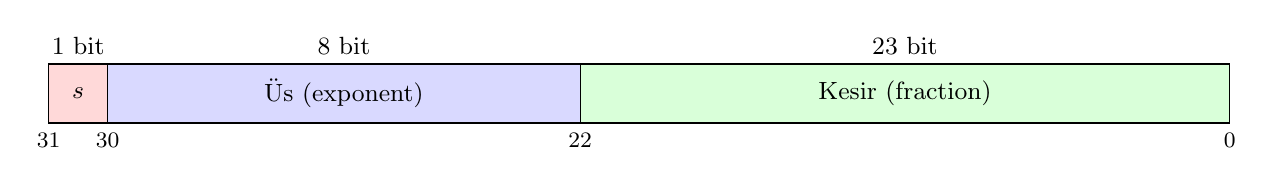
\begin{tikzpicture}[scale=0.75, every node/.style={font=\small}]
  % İşaret biti
  \draw[fill=red!15] (0,0) rectangle (1,1);
  \node at (0.5, 0.5) {$s$};
  \node[above] at (0.5, 1) {1 bit};
  % Üs alanı
  \draw[fill=blue!15] (1,0) rectangle (9,1);
  \node at (5, 0.5) {Üs (exponent)};
  \node[above] at (5, 1) {8 bit};
  % Kesir alanı
  \draw[fill=green!15] (9,0) rectangle (20,1);
  \node at (14.5, 0.5) {Kesir (fraction)};
  \node[above] at (14.5, 1) {23 bit};
  % Bit numaraları
  \node[below, font=\footnotesize] at (0, 0) {31};
  \node[below, font=\footnotesize] at (1, 0) {30};
  \node[below, font=\footnotesize] at (9, 0) {22};
  \node[below, font=\footnotesize] at (20, 0) {0};
\end{tikzpicture}
\caption{IEEE 754 tek duyarlı kayan nokta biçimi}
\label{fig:ieee754-tek}
\end{figure}

Sayının değeri şu formülle hesaplanır:
\begin{equation}
\text{değer} = (-1)^s \times 1{,}f \times 2^{(e - 127)}
\label{eq:ieee754}
\end{equation}
Burada $s$ işaret biti, $e$ üs alanının işaretsiz tam sayı değeri ve $f$ kesir alanıdır. Üs alanında 127 \textbf{kaydırması}\index{üs kaydırması} (İngilizcesi: \textit{bias}) kullanılır: saklanan $e$ değerinden 127 çıkarılarak gerçek üs elde edilir. $e = 127$ ise gerçek üs $0$, $e = 130$ ise gerçek üs $+3$, $e = 124$ ise gerçek üs $-3$ olur.

Kesir alanının solunda örtük bir ``$1,$'' bulunur (normalleştirilmiş sayılarda); bu sayede 23 bitlik kesir alanı aslında 24 bitlik bir doğruluk sağlar.

\subsection{Çift Duyarlı Gösterim (64 bit)}
\label{sec:ekA-ieee754-cift}

Daha yüksek doğruluk gereken uygulamalarda çift duyarlı (İngilizcesi: \textit{double precision}) gösterim kullanılır. Yapı tek duyarlı ile aynıdır; ancak üs alanı 11 bite, kesir alanı 52 bite çıkar ve kaydırma değeri 1023 olur.

\begin{table}[H]
\centering
\caption{IEEE 754 tek ve çift duyarlı gösterimlerin karşılaştırması}
\label{tab:ieee754-karsilastirma}
\begin{tabular}{lcc}
\toprule
\textbf{Özellik} & \textbf{Tek duyarlı} & \textbf{Çift duyarlı} \\
\midrule
Toplam bit sayısı & 32 & 64 \\
İşaret biti & 1 & 1 \\
Üs alanı & 8 bit & 11 bit \\
Kesir alanı & 23 bit & 52 bit \\
Üs kaydırması & 127 & 1023 \\
Üs aralığı & $-126$ ile $+127$ & $-1022$ ile $+1023$ \\
Yaklaşık onluk doğruluk & $\sim$7 basamak & $\sim$16 basamak \\
En küçük normalleştirilmiş & $\sim 1{,}2 \times 10^{-38}$ & $\sim 2{,}2 \times 10^{-308}$ \\
En büyük sonlu değer & $\sim 3{,}4 \times 10^{38}$ & $\sim 1{,}8 \times 10^{308}$ \\
\bottomrule
\end{tabular}
\end{table}

\subsection{Özel Değerler}
\label{sec:ekA-ieee754-ozel}

IEEE~754 standardı, olağan sayıların yanı sıra birkaç özel durumu da tanımlar:

\begin{table}[H]
\centering
\caption{IEEE 754 özel değerler (tek duyarlı)}
\label{tab:ieee754-ozel}
\begin{tabular}{ccl}
\toprule
\textbf{Üs ($e$)} & \textbf{Kesir ($f$)} & \textbf{Gösterilen değer} \\
\midrule
0       & 0       & $\pm 0$ (işaret bitine bağlı) \\
0       & $\neq 0$  & Denormalize sayı: $(-1)^s \times 0{,}f \times 2^{-126}$ \\
1--254  & herhangi  & Normalleştirilmiş sayı: $(-1)^s \times 1{,}f \times 2^{(e-127)}$ \\
255     & 0       & $\pm \infty$ (sonsuz) \\
255     & $\neq 0$  & NaN (sayı değil — \textit{Not a Number}) \\
\bottomrule
\end{tabular}
\end{table}

Sonsuz ($\infty$) değeri, sıfıra bölme gibi işlemlerin sonucu olarak ortaya çıkar. NaN ise $0/0$ veya $\sqrt{-1}$ gibi tanımsız işlemlerin sonucudur. Bu özel değerler sayesinde program çökmek yerine hesaplamaya devam edebilir ve hata daha sonra tespit edilebilir.

\begin{ornek}[A.21]
$-6{,}625$ sayısını IEEE~754 tek duyarlı biçimde gösterin.

\textbf{Çözüm:}

\textit{Adım 1 --- İşaret biti:} Sayı negatif olduğu için $s = 1$.

\textit{Adım 2 --- İkilik tabana çevirme:} $6 = (110)_2$; kesir kısmı: $0{,}625 = 0{,}5 + 0{,}125 = 2^{-1} + 2^{-3} = (0{,}101)_2$. Dolayısıyla $6{,}625 = (110{,}101)_2$.

\textit{Adım 3 --- Normalleştirme:} Noktayı sola kaydırarak $1{,}10101 \times 2^2$ elde edilir.

\textit{Adım 4 --- Üs hesabı:} Gerçek üs $= 2$; saklanan üs $= 2 + 127 = 129 = (10000001)_2$.

\textit{Adım 5 --- Kesir alanı:} Örtük 1 atılır, kalan $10101$ sağdan sıfırlarla 23 bite tamamlanır: $10101000000000000000000$.

Sonuç:
\[
\underbrace{1}_{s}\;\underbrace{10000001}_{e=129}\;\underbrace{10101000000000000000000}_{f} = \texttt{C0D40000}_{16}
\]
\end{ornek}

\begin{ornek}[A.22]
IEEE~754 tek duyarlı biçimde saklanan \texttt{41C80000}$_{16}$ değerinin onluk tabandaki karşılığını bulun.

\textbf{Çözüm:}

Onaltılık değeri ikilik tabana açalım:
\[
\texttt{41C80000}_{16} = 0\;10000011\;10010000000000000000000
\]
İşaret: $s = 0$ (pozitif). Üs: $e = (10000011)_2 = 131$; gerçek üs $= 131 - 127 = 4$. Kesir: $f = 10010\ldots$; örtük 1 ile: $1{,}1001$. Değer: $1{,}1001 \times 2^4 = 11001{,}0 = 16 + 8 + 1 = 25{,}0$. Sonuç: $+25{,}0$.
\end{ornek}

\begin{ornek}[A.23]
IEEE~754 tek duyarlı biçimde $0{,}1$ sayısını gösterin. Geri dönüşümde tam olarak $0{,}1$ elde edilir mi?

\textbf{Çözüm:}

$0{,}1$ sayısının ikilik tabandaki açılımı sonsuz yinelenen bir kesirdir:
\[
0{,}1_{10} = 0{,}0\overline{0011}\;0\overline{0011}\ldots_2
\]
Normalleştirme: $1{,}\overline{1001}\;1001\ldots \times 2^{-4}$. İşaret: $s = 0$. Üs: $-4 + 127 = 123 = (01111011)_2$. Kesir alanına 23 bit sığdırılır ve yuvarlanır. Sonuç:
\[
0\;01111011\;10011001100110011001101 = \texttt{3DCCCCCD}_{16}
\]
Geri dönüşümde elde edilen değer tam olarak $0{,}1$ değildir; yaklaşık $0{,}100000001490\ldots$ olur. Bu fark, kayan nokta aritmetiğinde \textbf{yuvarlama hatası}\index{yuvarlama hatası} olarak bilinir ve bilgisayar aritmetiğinin temel sınırlamalarından biridir.
\end{ornek}


% =====================================================
\section*{Alıştırmalar}
\addcontentsline{toc}{section}{Alıştırmalar}
\label{sec:ekA-alistirmalar}

\begin{alistirma}[\kolay]
$(54)_{10}$ sayısını ikilik, sekizlik ve onaltılık tabanda yazın.
\end{alistirma}

\begin{alistirma}[\kolay]
İkilik tabandaki $(11001110)_2$ sayısını onluk, sekizlik ve onaltılık tabanda yazın.
\end{alistirma}

\begin{alistirma}[\kolay]
Aşağıdaki 8 bitlik ikiye tümleyen sayıların onluk tabandaki karşılıklarını bulun: (a)~$01100100$, (b)~$10110011$, (c)~$11111111$, (d)~$10000000$.
\end{alistirma}

\begin{alistirma}[\kolay]
ASCII tablosunu kullanarak ``RISC-V'' dizgisinin her bir karakterinin onaltılık kodunu yazın.
\end{alistirma}

\begin{alistirma}[\kolay]
$(-23)_{10}$ sayısının 8 bitlik ikiye tümleyen gösterimini bulun. Sonucu onaltılık tabanda da ifade edin.
\end{alistirma}

\begin{alistirma}[\kolay]
3 bitlik Gray kodunu kullanarak $(5)_{10}$ sayısının Gray kodu karşılığını bulun.
\end{alistirma}

\begin{alistirma}[\orta]
8 bitlik ikiye tümleyen düzeninde aşağıdaki toplama işlemlerini yapın ve taşma olup olmadığını belirleyin: (a)~$64 + 53$, (b)~$(-80) + (-60)$, (c)~$100 + (-75)$.
\end{alistirma}

\begin{alistirma}[\orta]
4 bitlik bir ikiye tümleyen sisteminde gösterilebilecek en küçük ve en büyük tam sayıları belirleyin. 16 bit için aynı hesabı yineleyin.
\end{alistirma}

\begin{alistirma}[\orta]
$12{,}375$ sayısını IEEE~754 tek duyarlı kayan nokta biçiminde gösterin. Sonucu onaltılık tabanda da ifade edin.
\end{alistirma}

\begin{alistirma}[\orta]
IEEE~754 tek duyarlı biçimde saklanan \texttt{C1480000}$_{16}$ değerinin onluk tabandaki karşılığını bulun.
\end{alistirma}

\begin{alistirma}[\orta]
BCD düzeninde $49 + 38$ işlemini yapın. 4 bitlik her grubun sonucunu ayrı ayrı gösterin ve gerekli düzeltme adımlarını açıklayın.
\end{alistirma}

\begin{alistirma}[\orta]
``Öğüz'' kelimesinin UTF-8 kodlamasını onaltılık tabanda yazın. Her karakter için kaç bayt kullanıldığını belirtin. (İpucu: Ö = U+00D6, ğ = U+011F, ü = U+00FC, z = U+007A)
\end{alistirma}

\begin{alistirma}[\orta]
8 bitlik $01011010$ sayısını aşağıdaki her yöntemle yorumlayın ve onluk tabandaki karşılığını verin: (a)~işaretsiz, (b)~ayrı işaret biti, (c)~bire tümleyen, (d)~ikiye tümleyen.
\end{alistirma}

\begin{alistirma}[\orta]
$(-19)_{10}$ sayısını 8 bitlik ikiye tümleyen biçiminde bulun; ardından 16 bite işaretle genişletme uygulayın. Her iki gösterimin de onluk tabandaki değerinin aynı olduğunu doğrulayın.
\end{alistirma}

\begin{alistirma}[\zor]
IEEE~754 tek duyarlı biçimde $+\infty$, $-0$ ve NaN değerlerinin ikilik tabandaki gösterimlerini yazın.
\end{alistirma}

\begin{alistirma}[\zor]
IEEE~754 tek duyarlı biçimde gösterilebilecek, sıfırdan büyük en küçük normalleştirilmiş sayıyı ve en küçük denormalize sayıyı bulun. Bu iki değer arasındaki farkı açıklayın.
\end{alistirma}

\begin{alistirma}[\zor]
Birçok programlama dilinde \texttt{0.1 + 0.2 != 0.3} ifadesi doğru (true) sonuç verir. IEEE~754 tek duyarlı aritmetiğini kullanarak bu durumu açıklayın. $0{,}1$, $0{,}2$ ve $0{,}3$ sayılarının kayan nokta gösterimlerini karşılaştırın.
\end{alistirma}

\begin{alistirma}[\zor]
$n$ bitlik ikiye tümleyen düzeninde $-2^{n-1}$ sayısının ikiye tümleyenini almaya çalışın. Sonuç nedir ve bu neden bir sorun oluşturur?
\end{alistirma}
